\documentclass[11pt,a4paper]{article}

\usepackage[a4paper,margin=1in]{geometry}
\usepackage[T1]{fontenc}
\usepackage[utf8]{inputenc}
\usepackage{lmodern}
\usepackage{setspace}
\usepackage{hyperref}
\usepackage{xurl}
\usepackage{microtype}
\usepackage{graphicx}

\setstretch{1.0}
\urlstyle{tt}
\emergencystretch=2em

\title{Software Development Report}
\author{Brandon MacGillivray}
\date{27th April 2026}

\begin{document}

\hypersetup{pageanchor=false}
\begin{titlepage}
\centering
{\LARGE Software Development Report\par}
\vspace{1.5cm}
{\large An investigation into Lightweight Hand Pose estimation for Edge HCI\par}
\vspace{1cm}
{\large Brandon MacGillivray\par}
\vspace{0.5cm}
{\large 40321491\par}
\vspace{0.5cm}
{\large 27th April 2026\par}
\vfill
\end{titlepage}
\hypersetup{pageanchor=true}

\tableofcontents
\newpage

\section{Introduction}

This combined report covers two related software artefacts developed for the
project. The first is a research software repository that reconstructs and
evaluates a lightweight DRHand-inspired 2D hand pose estimation pipeline. The
second is a separate interactive demo application that uses live hand tracking
to present prepared visual outputs through gesture-based interaction.

\medskip

\noindent
The two artefacts were developed for different purposes and therefore have
different operational requirements, interfaces, and design constraints. The
research software is organised around reproducible command-line workflows for
training, evaluation, inference, and benchmarking, while the demo software is
organised around real-time camera input, gesture interpretation, and
presentation-oriented user interaction. For clarity, the two software reports
are presented separately within the same document.

\newpage
\section{Research Software Report}

\subsection{Purpose, Operation and Validation}

The software is intended to implement and evaluate a lightweight 2D hand pose
estimation pipeline for edge HCI, with a DRHand-inspired dual-branch model
that predicts hand keypoints from RGB images and supports training, inference,
benchmarking, and reproducible experiment reruns.

\medskip

\noindent The source repository for this software is available at
\url{https://github.com/Brandon-MacGillivray/CSC4006_research_software.git}.

\medskip

\noindent The primary persona for this software is a researcher working on
lightweight hand pose estimation who needs to train, evaluate, and reproduce
experiments from the repository.

\medskip

\noindent The main user stories for this software are:
\begin{itemize}
    \item ``As a researcher, I want to train the DRHand-inspired model on the
    supported datasets so that I can study its behaviour under different
    configurations.''
    \item ``As a researcher, I want to evaluate saved checkpoints and compare
    metrics so that I can judge model accuracy and robustness.''
    \item ``As a researcher, I want to rerun experiments from documented
    commands and preserved artefacts so that I can verify that the reported
    results are reproducible.''
    \item ``As a researcher, I want to run inference and generate qualitative
    outputs so that I can inspect the predicted hand keypoints visually.''
\end{itemize}

\noindent
A user operates the software from the command line by setting up the
documented Python environment, then running the repository scripts for the
required workflow, such as \path{scripts/train.py} for training,
\path{scripts/eval_metrics.py} for checkpoint evaluation, and
\path{scripts/predict_image.py} for single-image inference, with inputs and
options supplied as command-line arguments.

\medskip

\noindent
The software takes inputs such as dataset roots, checkpoint files, single RGB
images, model and evaluation settings passed through command-line arguments,
and it produces outputs such as trained checkpoint files, evaluation JSON
metrics, aggregated CSV result tables, benchmark summaries, and qualitative
prediction overlays or rendered figures.

\medskip

\noindent
A user can tell the software is working correctly when the lightweight test
suite passes, the main command-line scripts load and print valid help output,
and training, evaluation, inference, or benchmarking workflows execute
successfully and produce outputs in the expected format that can be compared
against the preserved reference JSON, CSV, checkpoint, and qualitative
artefacts bundled in the repository.

\subsection{Design and Implementation}

The software is implemented as a modular research artefact whose main design
goal is to separate reusable hand-pose functionality from workflow-specific
execution logic. Core behaviour is kept in the Python package under
\path{src/handpose}, while command-line scripts under \path{scripts/} provide
thin entry points for training, evaluation, inference, benchmarking,
aggregation, and qualitative rendering. This allows the same implementation to
support day-to-day experimentation, controlled reruns, and
assessment-oriented replication without duplicating logic across multiple
workflows.

\medskip

\noindent
Within the package, responsibilities are separated by concern rather than by
script. The \texttt{handpose.data} modules provide a common interface over the
supported datasets and keypoint layouts, \texttt{handpose.models} defines the
DRHand-inspired dual-branch network and its losses, \texttt{handpose.training}
contains the stage-specific optimisation and artefact logging code,
\texttt{handpose.inference} implements prediction and branch-fusion behaviour,
\texttt{handpose.evaluation} computes metrics and result payloads, and
\texttt{handpose.checkpoints} standardises checkpoint persistence and metadata
validation. This structure was intended to keep the codebase easier to test,
extend, and reuse across both the full 21-keypoint configuration and the
reduced 10-keypoint experiments.

\medskip

\noindent
At implementation level, the system is built around a small set of consistent
internal representations: resized RGB inputs, normalized keypoint
coordinates, metadata-rich checkpoints, and structured JSON or CSV outputs.
Dataset loaders convert dataset-specific annotations into a shared format, the
model produces heatmap and coordinate predictions, fused inference combines
these branches when required, and the surrounding scripts orchestrate complete
workflows such as training, evaluation, benchmarking, and result aggregation.
As a result, reproducibility is treated as part of the software design itself
rather than as an external add-on, with experiment definitions, preserved
checkpoints, and reference artefacts integrated directly into the repository.

\subsubsection{Significant Assumptions Made for the Design and Implementation}

The software assumes that the user has installed the supporting software
required for the intended workflow, including core dependencies and any
optional packages as defined in the documented installation and
replication instructions.

\medskip

\noindent
The software assumes that the user has access to the required datasets or
preserved artefacts in the directory structure expected by the repository
scripts.

\medskip

\noindent
The software assumes that the user has sufficient hardware resources for the
intended task. Smaller inference checks may be possible on CPU, but CUDA GPU
acceleration is strongly recommended for training and larger evaluation runs.

\medskip

\noindent
Framework equivalence. The software assumes that the DRHand method can be
reimplemented in PyTorch even though the original paper describes a TensorFlow
implementation. As a result, this repository should be understood as a
DRHand-inspired reconstruction rather than a strict reproduction, so exact
numerical agreement with the original paper should not be expected.

\medskip

\noindent
Heatmap supervision reconstruction. The software assumes Gaussian target
heatmaps for heatmap regression because the paper defines an L2 heatmap loss
but does not specify exactly how target heatmaps are constructed. This affects
optimisation because the heatmap branch is trained to match smooth Gaussian
peaks rather than some other target representation, which changes convergence
behaviour.

\medskip

\noindent
Effective batch-size reconstruction. The software assumes that the paper's
stage-2 batch size of 256 can be approximated using batch size 64 with
gradient accumulation on different hardware. This makes the training pipeline
usable on more limited systems, but it also means the repository reproduces
the paper's intended effective batch size only approximately rather than
literally.

\medskip

\noindent
No explicit augmentation policy. The software assumes a simple deterministic
preprocessing pipeline because the paper does not specify a detailed
augmentation strategy.

\medskip

\noindent
Visibility-aware evaluation assumption. The software assumes that evaluation
should mask invisible joints when visibility information is available. This
affects the reported metrics because performance is measured primarily on
visible landmarks, which may differ from alternative evaluation protocols.
This is a consequence of the annotation specifics of the RHD dataset. Where
often the coordinates of hands outside the image frame are still recorded.

\subsubsection{Languages, Packages, Frameworks, and Libraries Used}

Python. The software was built primarily in Python because it provides a
practical and widely used language for machine-learning research, rapid
experimentation, data processing, and command-line workflow development. This
made it suitable for implementing a research artefact that needed to support
training, evaluation, inference, benchmarking, and reproducibility.

\medskip

\noindent
MediaPipe. MediaPipe was used because the project included an explicit
baseline comparison against a strong lightweight hand-tracking system and also
relied on MediaPipe-related assets for pseudo-labelled or baseline-oriented
workflows. This choice was important because it gave the project a practical
reference point against a widely used real-time hand-pose system.

\medskip

\noindent
PyTorch. The main hand-pose pipeline was implemented in PyTorch because the
project required a flexible deep-learning framework for defining custom model
architectures, losses, and training procedures. PyTorch was particularly
suitable for this DRHand-inspired implementation because it allowed the
original dual-branch idea to be reconstructed clearly while remaining easy to
adapt for the reduced 10-keypoint and transfer-learning experiments.

\medskip

\noindent
PyTest. PyTest was used for automated testing because the repository needed a
lightweight way to verify important behaviour such as model output shapes,
fusion logic, and checkpoint validation. It was chosen to support software
quality assurance and to provide a quick validation route for assessors and
future users of the artefact.

\subsubsection{Overall Architecture / System Design and Interfaces Between Components}

\begin{figure}[htbp]
\centering
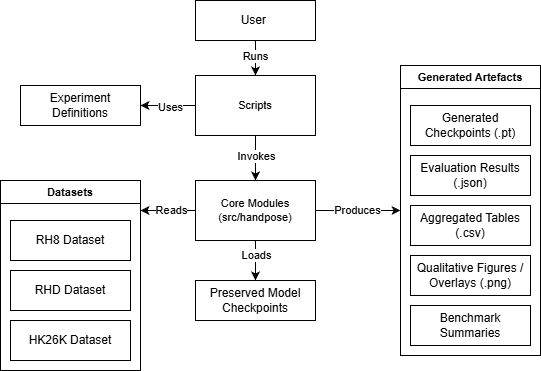
\includegraphics[width=0.7\textwidth]{4006_software_report-Page-2.drawio.png}
\caption{This figure shows the high-level architecture of the research software, including the main workflow scripts, core package modules, and artefact outputs.}
\label{fig:software-architecture}
\end{figure}

\begin{figure}[htbp]
\centering
\begin{minipage}[t]{0.60\textwidth}
\centering
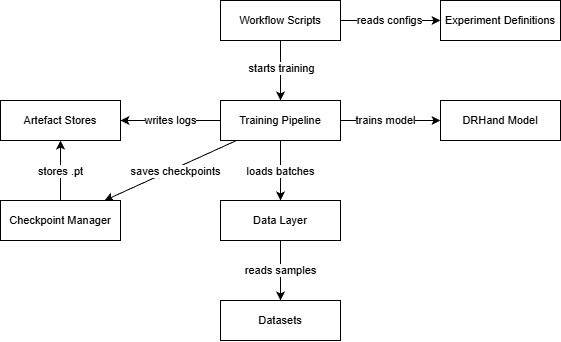
\includegraphics[width=\linewidth]{4006_software_report-comp_train_view.drawio.png}
\end{minipage}
\hfill
\begin{minipage}[t]{0.38\textwidth}
\centering
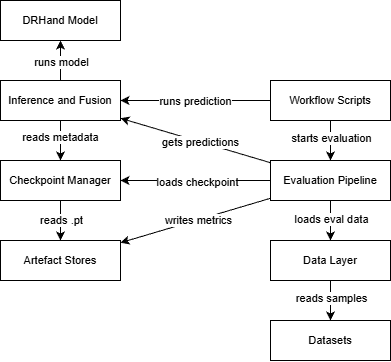
\includegraphics[width=\linewidth]{4006_software_report-comp_eval_view .drawio.png}
\end{minipage}
\caption{This figure shows the training and evaluation component views of the research software and the main interactions between workflow scripts, core modules, and artefact storage.}
\label{fig:training-evaluation-component-views}
\end{figure}

\begin{figure}[htbp]
\centering
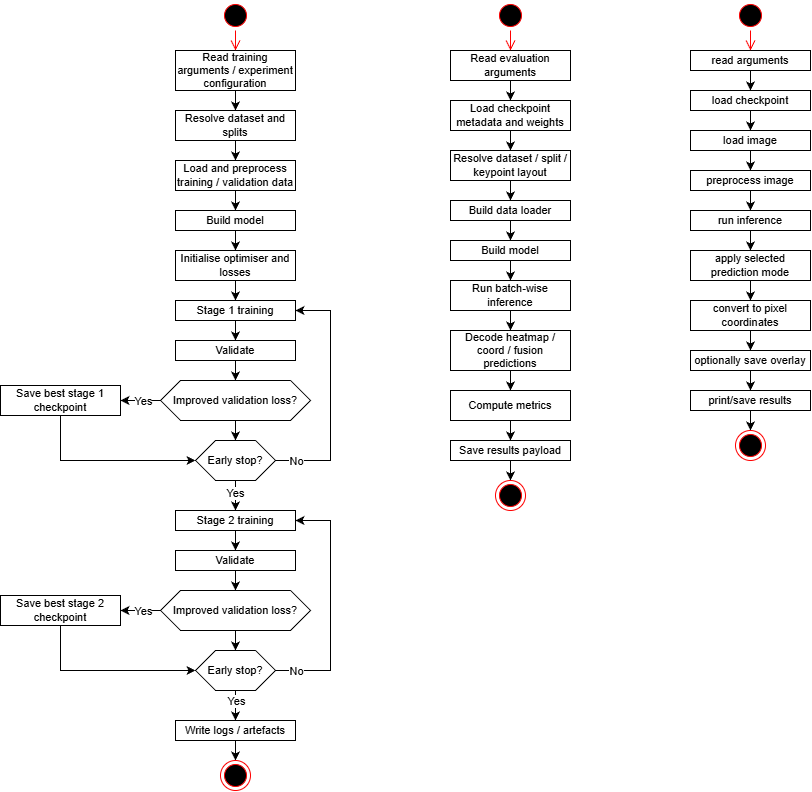
\includegraphics[width=1\textwidth,height=0.7\textheight,keepaspectratio]{4006_software_report-Page-4.drawio.png}
\caption{This figure shows the main training, evaluation, and inference activities and the order in which the repository workflows are executed.}
\label{fig:training-evaluation-activities}
\end{figure}

\paragraph*{Overall Structure}

Figure~\ref{fig:software-architecture} shows the overall system structure. The
repository is designed as a modular research artefact in which thin
command-line scripts provide the user-facing workflows, while the reusable
implementation is contained in the \path{src/handpose/} package. This
separates workflow orchestration from the core hand-pose logic and allows the
same internal code to support training, evaluation, benchmarking, and
single-image inference.

\medskip

\noindent
At the highest level, the user interacts with the software by running scripts
such as \path{scripts/train.py}, \path{scripts/eval_metrics.py}, and
\path{scripts/predict_image.py}. These scripts optionally use experiment
definitions and generated command files, then invoke the core modules
responsible for data loading, model execution, training, inference,
evaluation, and checkpoint handling.

\medskip

\noindent
The core modules read dataset files from disk and produce new artefacts such
as trained checkpoints, evaluation JSON files, aggregated CSV tables,
benchmark summaries, and qualitative figures. This structure keeps the
execution interface simple while ensuring that the main implementation remains
reusable and consistent across workflows.

\paragraph*{Training View}

Figure~\ref{fig:training-evaluation-component-views} expands this design into
separate training and evaluation component views. In the training view, the
workflow scripts start the training pipeline, which requests batches from the
data layer, passes them through the DRHand model, computes the required
losses, and updates the model parameters.

\medskip

\noindent
The data layer provides a shared interface for loading and preprocessing
supported datasets into normalized tensor representations. During training,
the checkpoint manager validates and saves model state together with metadata,
while the training pipeline also writes logs and loss histories to the
artefact store.

\paragraph*{Evaluation and Inference View}

In the evaluation and inference view, the workflow scripts start either
checkpoint evaluation or direct prediction. The evaluation pipeline loads a
saved checkpoint through the checkpoint manager, rebuilds the model
configuration, obtains evaluation samples from the data layer, and requests
predictions from the inference and fusion module.

\medskip

\noindent
That module runs the DRHand model, decodes heatmap outputs, uses the
coordinate branch predictions, and applies the fusion rule when fused
inference is requested.

\medskip

\noindent
The resulting predictions are then used by the evaluation pipeline to compute
metrics such as SSE, EPE, PCK, timing information, and optional fusion
diagnostics, which are written back to the artefact store as structured
outputs.

\paragraph*{Workflow Activities}

Figure~\ref{fig:training-evaluation-activities} complements the component
views by showing the workflows as activities. It emphasizes the execution
order of the main repository tasks: training moves from dataset loading and
preprocessing to staged optimisation, validation, and checkpoint export,
while evaluation and inference move from checkpoint loading and sample
preparation to prediction, fusion, metric computation, and output generation.

\paragraph*{Interfaces Between Components}

The interfaces between these components are mainly file-based and
tensor-based. File-based interfaces include dataset roots, annotation files,
checkpoint \texttt{.pt} files, evaluation \texttt{.json} outputs, summary
\texttt{.csv} files, and rendered \texttt{.png} figures.

\medskip

\noindent
In-memory interfaces are primarily PyTorch tensors representing images,
keypoint coordinates, visibility values, heatmaps, and predicted coordinates.
Checkpoint metadata provides an additional interface between workflows by
preserving information such as training stage, epoch, keypoint layout, and
other configuration details needed to reload and evaluate a model correctly.

\subsubsection{Data Model(s), Including In-Memory Structures and Persistent Storage}

\paragraph*{Processed Data}

The main inputs are RGB hand images and per-image annotations from the
supported datasets, including 2D keypoint coordinates and visibility values.
During preprocessing, these inputs are converted into a shared tensor
representation that is reused across training, evaluation, and inference.

\paragraph*{In-Memory Representation}

The main in-memory structures are image tensors of shape \texttt{(C,H,W)},
keypoint-coordinate tensors of shape \texttt{(K,2)}, visibility tensors of
shape \texttt{(K)}, predicted heatmaps of shape \texttt{(K,64,64)}, and
predicted coordinate tensors of shape \texttt{(K,2)}.

Where C denotes the number of image channels, H and W denote image height and
width, K denotes the number of keypoints, and N denotes batch size. The model
uses RGB inputs, so typically C = 3, and the predicted heatmaps have spatial
size 64 x 64.

\paragraph*{Persistent Storage}

Persistent storage in the repository is file-based. Source datasets remain on
disk as image and annotation files, while intermediate and final outputs are
saved as experiment artefacts. Training checkpoints are written as PyTorch
\texttt{.pt} files containing model state and metadata, loss histories are
stored as CSV, evaluation outputs are written as JSON, aggregated summaries
are stored as CSV, and qualitative overlays or rendered figures are exported
as \texttt{.png}. This design supports reproducibility because trained states,
metrics, and generated figures can all be reloaded or compared directly from
the filesystem.

\medskip

\begin{table}[htbp]
\centering
\small
\begin{tabular}{|p{0.22\textwidth}|p{0.34\textwidth}|p{0.22\textwidth}|}
\hline
\textbf{Data item} & \textbf{In-memory form} & \textbf{Persistent form} \\
\hline
RGB input image & Preprocessed tensor \texttt{(3,H,W)} & \texttt{.png} or \texttt{.jpg} image files \\
\hline
Ground-truth hand pose & Keypoint tensor \texttt{(K,2)} plus visibility tensor \texttt{(K)} & RHD annotations or COCO-style \texttt{.json} annotations \\
\hline
Training / evaluation batch & Batched tensors such as \texttt{(N,3,H,W)} and \texttt{(N,K,2)} & Runtime only; constructed by data loaders \\
\hline
Model predictions & Heatmaps \texttt{(N,K,64,64)} and coordinates \texttt{(N,K,2)} & Exported prediction or metric payloads in \texttt{.json}; optional qualitative \texttt{.png} outputs \\
\hline
Checkpoint state & Python dict containing \texttt{model\_state}, keypoint layout, stage, epoch, and training metadata & PyTorch checkpoint \texttt{.pt} files \\
\hline
Result summaries & Scalar metrics and aggregated experiment statistics & CSV tables and JSON result files \\
\hline
\end{tabular}
\caption{This table summarises the main data representations used by the repository, including their in-memory forms and persistent storage formats.}
\label{tab:data-representations}
\end{table}

\subsubsection{Significant Methods, Functions, or Other Lower-Level Elements}

\paragraph*{Core Model}

The most important lower-level implementation element is
\texttt{HandPoseNet} in \path{src/handpose/models/hand_pose_model.py}, which
acts as the main wrapper around the learned model.

\medskip

\noindent
It combines the shared backbone, heatmap regression head, and coordinate
regression head into one interface and provides the forward paths used during
both training and inference. This makes it the central model component on
which the rest of the repository depends.

\paragraph*{Architecture and Optimisation}

At the architectural level, the most significant lower-level classes are
\texttt{Backbone}, \texttt{Heatmap\_reg}, and \texttt{coord\_reg} in
\path{src/handpose/models/architecture.py}, together with the reusable block
definitions in \path{src/handpose/models/block.py}.

\medskip

\noindent
These classes implement the shared feature extractor, the heatmap branch, the
coordinate branch, and the depthwise-separable and upsampling building blocks
from which the DRHand-inspired model is assembled.

\medskip

\noindent
The most important optimisation-related functions are
\texttt{coords\_to\_heatmaps}, \texttt{HeatmapMSELoss}, and \texttt{WingLoss}
in \path{src/handpose/models/losses.py}, along with
\texttt{build\_optimizer\_stage1}, \texttt{build\_optimizer\_stage2},
\texttt{train\_one\_epoch}, and \texttt{validate} in the training modules.

These functions define how supervision targets are constructed, how the two
training losses are computed, how different stages of the model are
optimised, and how batch-wise training and validation are carried out.

\paragraph*{Data Processing and Fusion}

Another important group of lower-level functions appears in the preprocessing
and dataset-loading code. The dataset factory and dataset classes in
\path{src/handpose/data/} provide a unified interface for loading RHD and
COCO-style hand datasets, while preprocessing helpers in
\path{src/handpose/data/transforms.py} resize images, convert them to
tensors, and rescale keypoint coordinates. These functions are significant
because all training, evaluation, and inference workflows depend on the same
shared input format.

\medskip

\noindent
The lower-level functions implementing branch fusion. In
\path{src/handpose/inference/fusion.py}, functions such as
\texttt{heatmaps\_to\_coords\_argmax}, \texttt{resolve\_fusion\_bone\_edges},
and \texttt{fuse\_coords} define how heatmap predictions are decoded and how
the final fused prediction is selected from the heatmap and coordinate
branches. These functions are central because the fusion rule is one of the
defining design features of the implemented pipeline.

\paragraph*{Checkpointing and Workflow Entry Points}

Checkpoint and evaluation handling. Functions in
\path{src/handpose/checkpoints.py} define how checkpoints are validated,
saved, and reloaded, while \texttt{evaluate\_checkpoint} in
\path{src/handpose/evaluation/eval_metrics_core.py} performs the main metric
computation for SSE, EPE, PCK, timing, and optional fusion diagnostics. These
components are important because they make the repository reproducible and
allow trained models to be reused consistently across training, inference, and
result generation workflows.

\medskip

\noindent
The user-facing scripts under \path{scripts/} are thin but important workflow
connectors. Scripts such as \texttt{train.py}, \path{eval_metrics.py},
\path{predict_image.py}, and \path{benchmark_pipeline.py} do not contain the
main modelling logic themselves, but they are the main entry points through
which a user accesses the lower-level implementation for complete training,
evaluation, inference, and benchmarking tasks.

\subsubsection{Important Errors and Their Conditions}

\paragraph*{Input and Configuration Errors}

Several important errors in the software are caused by invalid inputs,
missing files, or inconsistent configuration between artefacts. For example,
the checkpoint utilities raise errors when a checkpoint is missing required
metadata fields, has a mismatched keypoint layout, contains duplicate
keypoint indices, or uses an unsupported checkpoint version. Similar
validation errors occur when invalid keypoint subsets are requested, when
unsupported dataset names or split aliases are supplied, or when an invalid
prediction mode or negative PCK threshold is passed on the command line. In
these cases, the software responds by raising a clear \texttt{ValueError} and
stopping execution rather than continuing with inconsistent state.

\paragraph*{Runtime Resource Errors}

A second group of important errors occurs when required runtime resources are
not available. Examples include missing dataset directories, missing image
files, empty evaluation image folders, failed imports of optional
dependencies such as MediaPipe, or requesting CUDA on a machine where it is
not available. These conditions are handled through exceptions such as
\texttt{FileNotFoundError} or \texttt{RuntimeError}. The software does not
silently ignore these problems; instead, it fails early and reports the
missing dependency, missing path, or unsupported device condition so that the
user can correct the environment before rerunning the workflow.

\paragraph*{Workflow State Errors}

Further errors can arise from invalid workflow state during training or
evaluation. For example, stage-specific training functions raise errors if an
unsupported stage number is used, if gradient accumulation is configured with
an invalid value, or if stage 2 is requested without the required coordinate
loss. Training also raises an error if \texttt{--skip-stage1} is used without
providing an initial checkpoint.

\medskip

\noindent
Evaluation and qualitative-rendering workflows can also fail when no samples
match the requested dataset split or when the selected checkpoint does not
contain the keypoints required for shared-10 evaluation or fusion. In these
situations, the software again responds by terminating with an explicit error
message, which helps prevent silent misuse of the repository and makes
debugging more straightforward.

\subsubsection{User Interface Design}

\paragraph*{Command-Line Interaction}

The user interacts with the software primarily through a command-line
interface. The main workflows are exposed as separate Python scripts under
\path{scripts/}, including training, evaluation, benchmarking, single-image
inference, qualitative rendering, and result aggregation.

\medskip

\noindent
In practice, the user runs these scripts from the repository root, supplies
the required paths and options as command-line arguments, and receives outputs
such as checkpoints, JSON result files, CSV summaries, printed metrics, or
rendered visualisations.

\medskip

\noindent
This command-line design was chosen because the software is a research
artefact rather than an end-user application. The main tasks involve running
controlled experiments, reproducing reported results, evaluating checkpoints
under different conditions, and generating analysis artefacts.

\medskip

\noindent
These activities are better supported by explicit script arguments than by a
graphical user interface, because command-line workflows are easier to
document, automate, reproduce, and integrate with local machines, Conda
environments, and HPC or Slurm-based execution.

\paragraph*{Separation of Interface and Core Logic}

Another important interface choice was to separate the reusable
implementation from the user-facing entry points. The core logic is
implemented in the \path{src/handpose/} package, while the scripts act as
thin workflow wrappers around that logic. This was done so that the user
interface remains simple at the script level while the lower-level code
remains modular and reusable. As a result, users can run complete workflows
through a small number of documented commands without needing to interact
directly with the internal package structure.

\paragraph*{Explicit Runtime Configuration}

The interface relies on explicit file and path arguments for datasets,
checkpoints, and output locations. This choice was made to keep the
repository portable across different machines and storage layouts, especially
since some datasets are external and not bundled with the artefact. By
making these dependencies explicit at runtime, the software avoids hard-coding
machine-specific paths and makes the execution process clearer for assessors
and future users.

\subsubsection{Quality Assurance Steps}

\paragraph*{Documentation and Artefact Management}

Maintainability was further supported through reproducibility-oriented
documentation and artefact management. The repository includes installation
instructions, requirement notes, a replication guide, curated experiment
command files, preserved checkpoints, and saved result artefacts. These were
important quality-assurance measures because they made the software easier to
inspect, rerun, and extend, while also ensuring that the reported
experimental outputs could be traced back to concrete workflows within the
repository.

\paragraph*{Version Control and Versioning}

Version control was used throughout development by maintaining the project as
a Git-based repository. This allowed the software, documentation, experiment
definitions, and preserved artefacts to be developed within a single
structured history rather than as disconnected files. Using version control
was important because the project involved repeated changes to model design,
training configuration, evaluation workflows, reporting artefacts, and
supporting documentation, all of which needed to remain traceable over time.

\medskip

\noindent
Changes were tracked and managed through the normal Git workflow of recording
edits to the repository as development progressed. This made it possible to
monitor the evolution of scripts, source modules, experiment files, and paper
materials, and helped prevent important changes from being lost or mixed
together without record. It also supported safer experimentation, since
alternative implementations or revised configurations could be introduced
while preserving the earlier state of the project.

\paragraph*{Code Style and Convention}

The code follows a consistent Python style based on clear module separation,
descriptive function names, and lightweight internal documentation. The
repository is organised by responsibility, with separate modules for data
loading, model definition, training, inference, evaluation, and checkpoint
handling. Within these modules, functions and classes generally use
descriptive \texttt{snake\_case} naming for functions and variables, and
class-based naming for model components such as \texttt{HandPoseNet}. This
made the code easier to navigate because related logic was grouped together
rather than scattered across large scripts.

\medskip

\noindent
A consistent convention was also followed for docstrings and purpose
statements. Most modules begin with a short summary docstring explaining
their role in the repository, and most important functions include concise
docstrings describing what they do. This helped keep the code clear because
users and future readers can understand the role of a file or function
without having to infer it entirely from implementation details.

\medskip

\noindent
The code also follows a convention of keeping user-facing workflow logic
separate from reusable implementation logic. Scripts under \path{scripts/}
mainly parse arguments and call functions from the \path{src/handpose/}
package, while the package itself contains the lower-level logic. This
convention improved consistency because training, evaluation, inference, and
benchmarking were all built on shared internal code rather than separate
duplicated implementations.

\medskip

\noindent
The use of explicit validation and informative error messages at key
interfaces. Functions that depend on specific assumptions, such as checkpoint
schema, prediction modes, dataset names, keypoint layouts, or device
availability, usually check these conditions directly and raise clear
exceptions if they are violated. This kept the behaviour of the software more
predictable and made the codebase easier to maintain, since failures tended to
occur close to the source of the problem rather than emerging later as
ambiguous downstream bugs.

\paragraph*{Automated Testing}

The repository includes a lightweight automated test suite implemented with
\texttt{pytest}. These tests provide a fast validation layer before running
more expensive workflows such as full training or dataset-based evaluation.

\medskip

\noindent
\texttt{test\_hand\_pose\_net\_output\_shapes} in
\path{tests/test_model_shapes.py}. This test instantiates
\texttt{HandPoseNet} for both the standard 21-keypoint layout and the reduced
10-keypoint layout, passes a dummy tensor of shape \texttt{(2,3,256,256)}
through the model, and checks that the outputs have shapes
\texttt{(2,K,64,64)} for heatmaps and \texttt{(2,K,2)} for coordinates. It
also checks that the returned tensors contain only finite values. This
verifies the most basic output-shape contract of the model.

\medskip

\noindent
\texttt{test\_heatmaps\_to\_coords\_argmax\_decodes\_normalized\_xy} in
\path{tests/test_fusion.py}. This test constructs a small heatmap with a
known maximum location and checks that \texttt{heatmaps\_to\_coords\_argmax}
returns the expected normalized coordinate. The same file also includes
\texttt{test\_resolve\_fusion\_bone\_edges\_supports\_tip\_base\_10\_and\_rejects\_other\_layouts},
which checks that supported keypoint layouts are accepted while unsupported
layouts raise a \texttt{ValueError}. These tests verify both correct fusion
behaviour and correct rejection of invalid inputs.

\medskip

\noindent
\texttt{test\_validate\_checkpoint\_accepts\_and\_normalizes\_valid\_schema}
in \path{tests/test_checkpoints.py}. This test supplies checkpoint metadata
with string values for stage and epoch and checks that validation normalizes
them correctly. The same file also includes
\texttt{test\_validate\_checkpoint\_rejects\_duplicate\_keypoint\_indices}
and \texttt{test\_validate\_checkpoint\_rejects\_inconsistent\_num\_keypoints},
which confirm that malformed checkpoint metadata is rejected. These tests
protect the checkpoint contract used by training, evaluation, and inference
workflows.

\clearpage

\section{Demo Software Report}

\subsection{Purpose, Operation and Validation}

\noindent This software is a gesture-driven interactive demo developed for
live presentation. Its purpose is to allow a demo user to explore prepared
visual outputs through direct hand interaction rather than through
command-line experiments or conventional desktop controls.

\medskip

\noindent The source repository for this software is available at
\url{https://github.com/Brandon-MacGillivray/CSC4006_demo_software.git}.

\medskip

\noindent The primary user story for this demo is: ``As a demo user, I want
to control the demo through hand gestures so that I can navigate the showcase
and inspect the prepared visual outputs without relying on a mouse or
keyboard.''

\medskip

\noindent In operation, the demo opens the ZED camera, detects one hand, and
uses the tracked hand as the main control input. Palm movement is used to
drive an on-screen cursor, while a fist gesture is interpreted as a click.
Through this interaction model, the user can move from the start page to the
menu and then select either the segmentation demonstration or the tone-mapping
demonstration.

\medskip

\noindent The software can be considered to be working correctly when it
starts successfully, detects the camera, shows stable cursor movement in
response to hand motion, registers fist gestures as intended selections,
allows the user to navigate the demonstration pages correctly, and updates the
visual outputs in the expected way.

\subsection{Design and Implementation}

\subsubsection{Significant Assumptions Made for the Design and Implementation}

This demo assumes that a working ZED camera is connected and available at
runtime, that a single hand can be tracked reliably enough for
gesture-based interaction, that the application is used in its intended
portrait presentation layout, that the required segmentation and tone-mapping
assets are already present locally, and that the application is launched from
the expected working directory so that its relative asset paths resolve
correctly during execution.

\subsubsection{Languages, Packages, Frameworks, and Libraries Used}

The demo was implemented in Python 3.10, with PySide6 used for the graphical
user interface, MediaPipe used for hand tracking, and \texttt{pyzed} used for
interaction with the ZED camera. With support from OpenCV, Pillow and NumPy.

\subsubsection{Overall Architecture / System Design and Interfaces Between Components}

The demo was implemented as a small interactive architecture with three main
parts. First, a perception pipeline acquires frames from the ZED camera,
preprocesses them, and applies MediaPipe Hands to estimate landmarks from
which cursor position, palm width, and fist-click state are derived. Second,
a central \texttt{MainWindow} acts as the controller for the application: it
receives pose updates, maintains the active page, updates the overlay, routes
gesture-derived click events to the appropriate page logic, and triggers
timeout recovery when tracking is lost. Third, the presentation layer is
implemented as a set of pages for the start screen, menu, segmentation
demonstration, and tone-mapping demonstration, with the content pages loading
prepared visual assets from disk.

\medskip

\noindent
This structure was chosen because it separates latency-sensitive vision
processing from presentation logic while still allowing both demonstrations to
share the same interaction controller. The perception pipeline is responsible
for deriving interaction state from live camera input, the controller manages
application state and gesture routing, and the presentation layer is
responsible for what the user sees. This separation reduces coupling between
different responsibilities, helps keep the interface responsive during live
use, and makes the overall flow of interaction easier to understand.

\medskip

\noindent
Alternative designs were possible. For example, camera acquisition, hand
tracking, and page behaviour could have been implemented directly inside the
GUI event loop or combined within a more monolithic single-class design.
However, this approach was not chosen because it would have made the
application more tightly coupled, harder to reason about, and more likely to
become unresponsive during live interaction. The adopted design was thus more
appropriate for a demo that depended on real-time tracking and clear
separation between interaction logic and presentation behaviour.

\medskip

\begin{figure}[htbp]
\centering
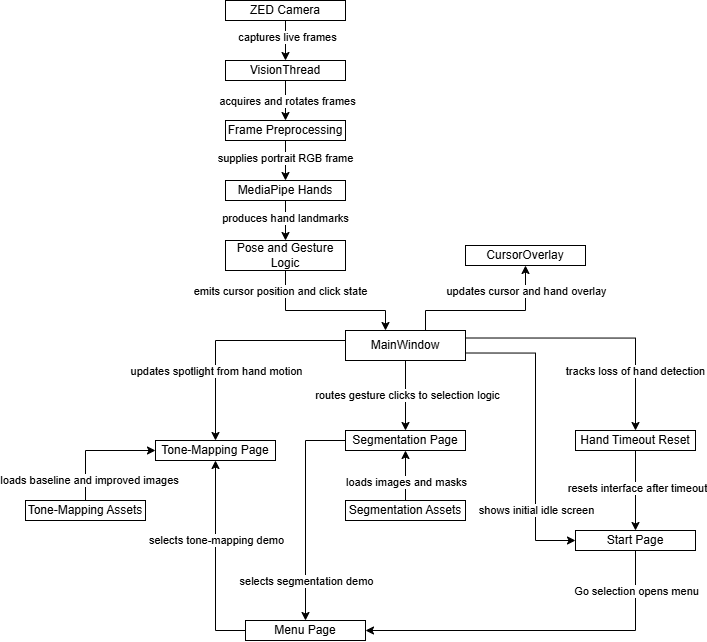
\includegraphics[width=0.95\textwidth]{4006_software_report-demo_diagram.drawio.png}
\caption{Architecture of the interactive demo, showing the live hand-tracking pipeline, central window controller, and gesture-driven demo pages.}
\label{fig:interactive-demo-architecture}
\end{figure}

\subsubsection{Data Model(s), Including In-Memory Structures and Persistent Storage}

The main runtime inputs are frames from the ZED camera together with locally
stored microscopy images, masks, and tone-mapped image pairs. In memory,
these are represented as image buffers, hand-tracking outputs, cursor and
gesture state, connected-component overlays for the segmentation
demonstration, and fixed baseline or improved image pairs for the
tone-mapping demonstration. Persistent storage is file-based rather than
database-based.

\medskip

\noindent
This data model was chosen because it matched the role of the demo as a live
presentation tool rather than as a general-purpose software platform. The
application needed to combine real-time camera input with a small set of
prepared assets and transform them into responsive visual behaviour with as
little overhead as possible. A lightweight in-memory representation was
therefore appropriate, while file-based storage was sufficient because the
demo uses a fixed asset set and does not need complex persistence, remote
access, or long-term state management.

\medskip

\noindent
Alternative designs were possible. For example, the prepared assets could
have been managed through a more elaborate asset-management layer or a
database-backed store. The visual outputs could also have been generated
dynamically rather than being read from prepared files. These approaches were
not adopted because they would have introduced additional complexity without
clear benefit for a demo whose purpose was to present fixed prepared outputs
through gesture-based interaction. The simpler file-based and in-memory
approach was therefore the more suitable design for this software.

\subsubsection{Significant Methods, Functions, or Other Lower-Level Elements}

The most significant lower-level elements in this demonstrator are the helper
functions and classes that convert hand landmarks into usable interaction
behaviour. Functions such as \texttt{palm\_center}, \texttt{palm\_width},
\texttt{tip\_mcp\_norm}, and \texttt{is\_fist} in
\path{mp_handpose_demo/hand_18.py} are important because they define how the
software derives cursor position, hand scale, and click-like gesture state
from the tracked hand landmarks.

\medskip

\noindent
The \texttt{VisionThread} class performs live camera acquisition, frame
preprocessing, MediaPipe hand tracking, and click debouncing before emitting
pose updates to the rest of the application, forming the main runtime bridge
between raw camera input and the higher-level gesture-driven behaviour seen by
the user.

\medskip

\noindent
The presentation behaviour of the demonstrator is implemented mainly through
\texttt{CursorOverlay}, \texttt{SegmentationDemoWidget},
\texttt{MultiMaskSegmentationWidget}, and \texttt{ToneMappingDemoWidget}.
These classes are significant because they implement the visible behaviour of
the two demonstrations: drawing the live overlay, resolving clicked
segmentation regions, revealing RNvU masks, and displaying the hand-controlled
tone-mapping spotlight. The \texttt{MainWindow} class coordinates these
components and routes the gesture-derived events that connect tracking input
to page behaviour.

\subsubsection{Important Errors and Their Conditions}

The software may fail to start correctly if the ZED camera is not connected,
cannot be opened, or is otherwise unavailable at runtime. Parts of the
demonstrator may fail or display incomplete behaviour if required images or
mask files are missing, unreadable, or empty. Because the implementation uses
relative asset paths, the software also depends on being launched from the
expected working directory so that those paths resolve correctly. Even when
the application starts successfully, behaviour may degrade if the user's hand
is not tracked reliably, if gesture detection is unstable, or if tracking is
lost during use. Under these conditions, cursor motion may become unstable,
intended selections may not register correctly, or the interface may return
to the start screen after the configured timeout.

\subsubsection{User Interface Design}

The interaction logic is implemented explicitly rather than through a generic
gesture library. The cursor position is derived from the mean position of a
small set of palm-related landmarks, mirrored horizontally to match user
expectation, and then smoothed before being displayed so that motion appears
stable rather than jittery. A fist is detected by comparing
fingertip-to-base distances against palm width, and clicks are debounced so
that one closing motion does not trigger repeated activations. If no hand is
detected for a short timeout period, the interface automatically returns to
the start screen, which helps recover from tracking loss during live use. In
practical terms, this gives the demo two forms of interaction: continuous
hand motion is used to control cursor-like behaviour, while discrete fist
closures are used as selection events for navigation and page-specific
actions.

\medskip

\noindent
The first demonstration is event-driven. It presents microscopy imagery
together with precomputed segmentation data, and a user selection event
determines which prepared overlay is revealed. In one mode, a binary mask is
converted into connected components and the selected component is highlighted
when the user clicks on the image. In another mode, multiple precomputed RNvU
retina masks are loaded and the mask covering the selected pixel is revealed.

\medskip

\noindent
The second demonstration is continuous rather than event-driven. It presents
tone-mapping results using paired images: a baseline image is shown across the
whole display, while an improved image is revealed only inside a
hand-controlled spotlight. The spotlight position follows the
gesture-controlled cursor and its radius scales with palm width, so hand
motion acts as a live control input rather than as a sequence of clicks. In
both demonstrations, the software does not run segmentation or tone-mapping
models live. It instead provides an interaction layer for exploring prepared
outputs visually.

\medskip

\noindent
Representative screenshots of the implemented user interface are shown in
Figure~\ref{fig:ui-screens}.

\begin{figure}[htbp]
    \centering
    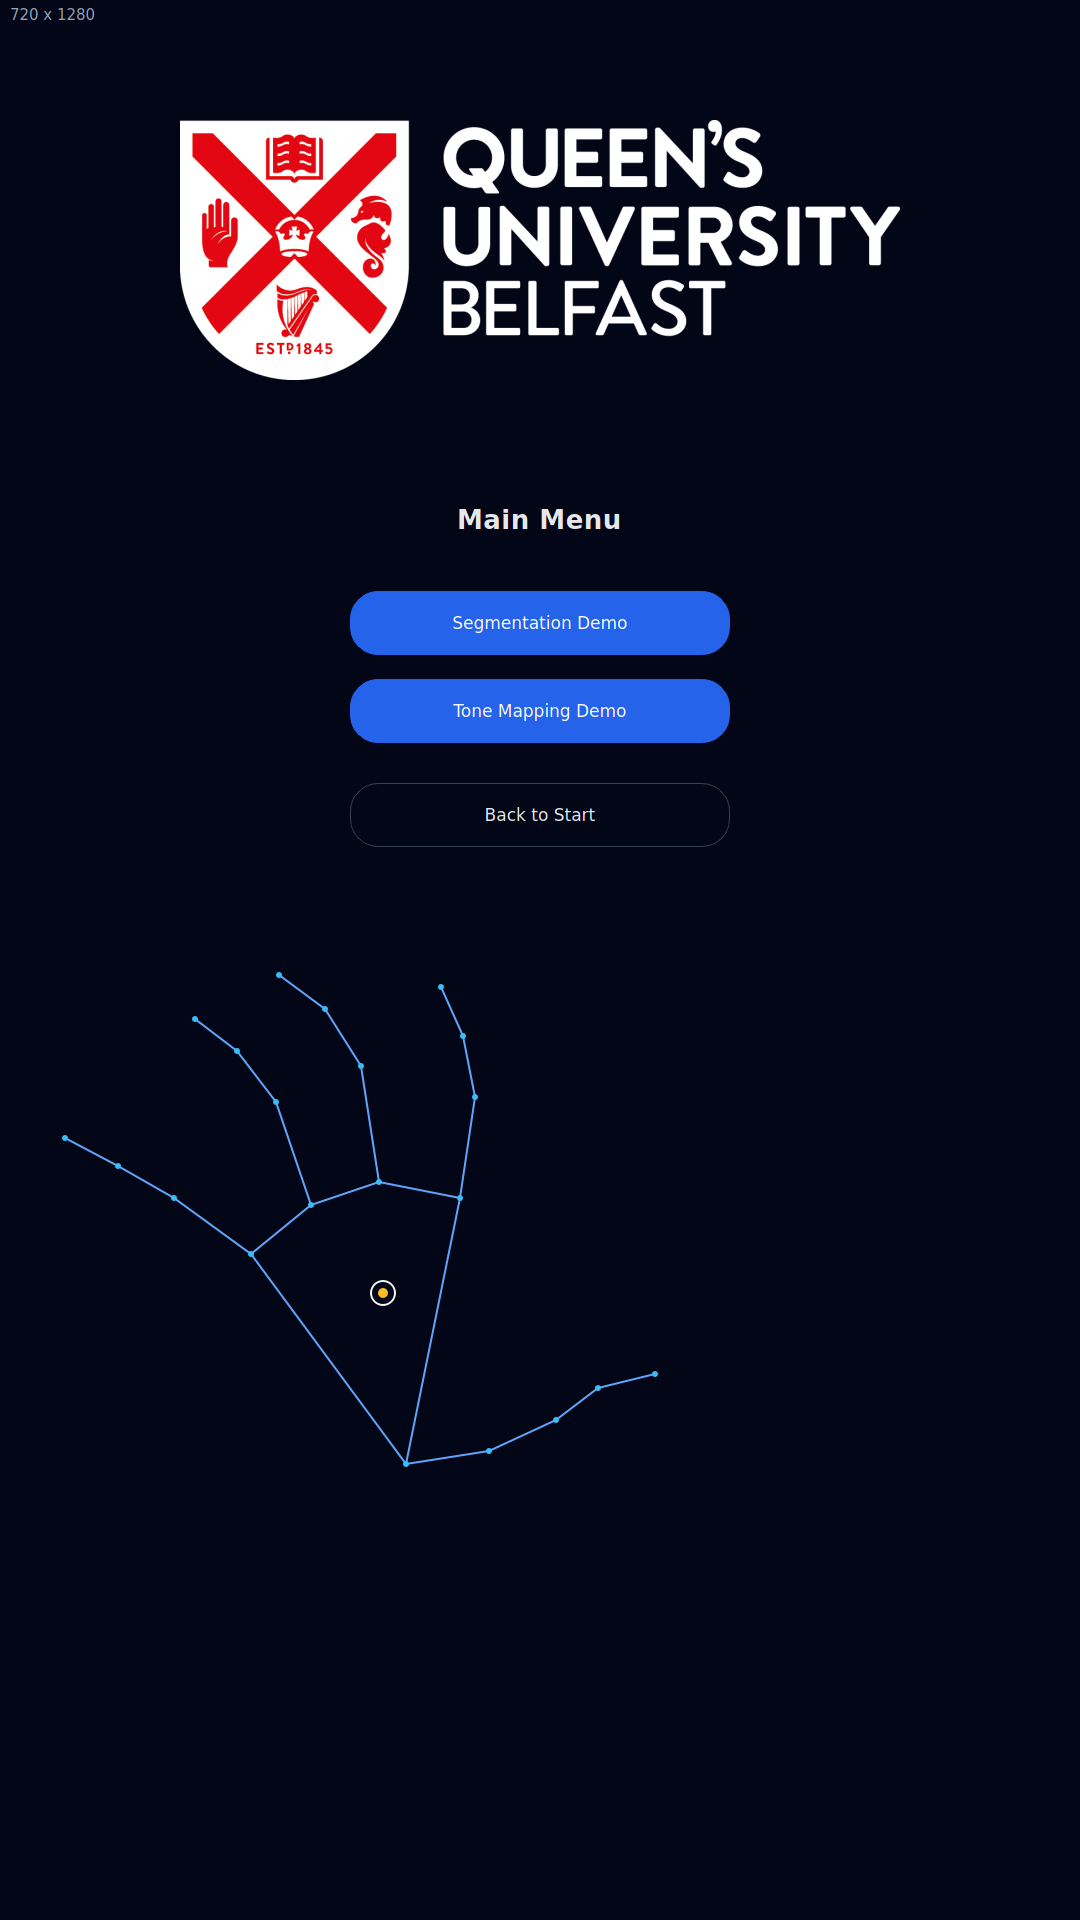
\includegraphics[width=0.31\textwidth]{Screenshot from 2026-04-23 21-32-25.png}
    \hfill
    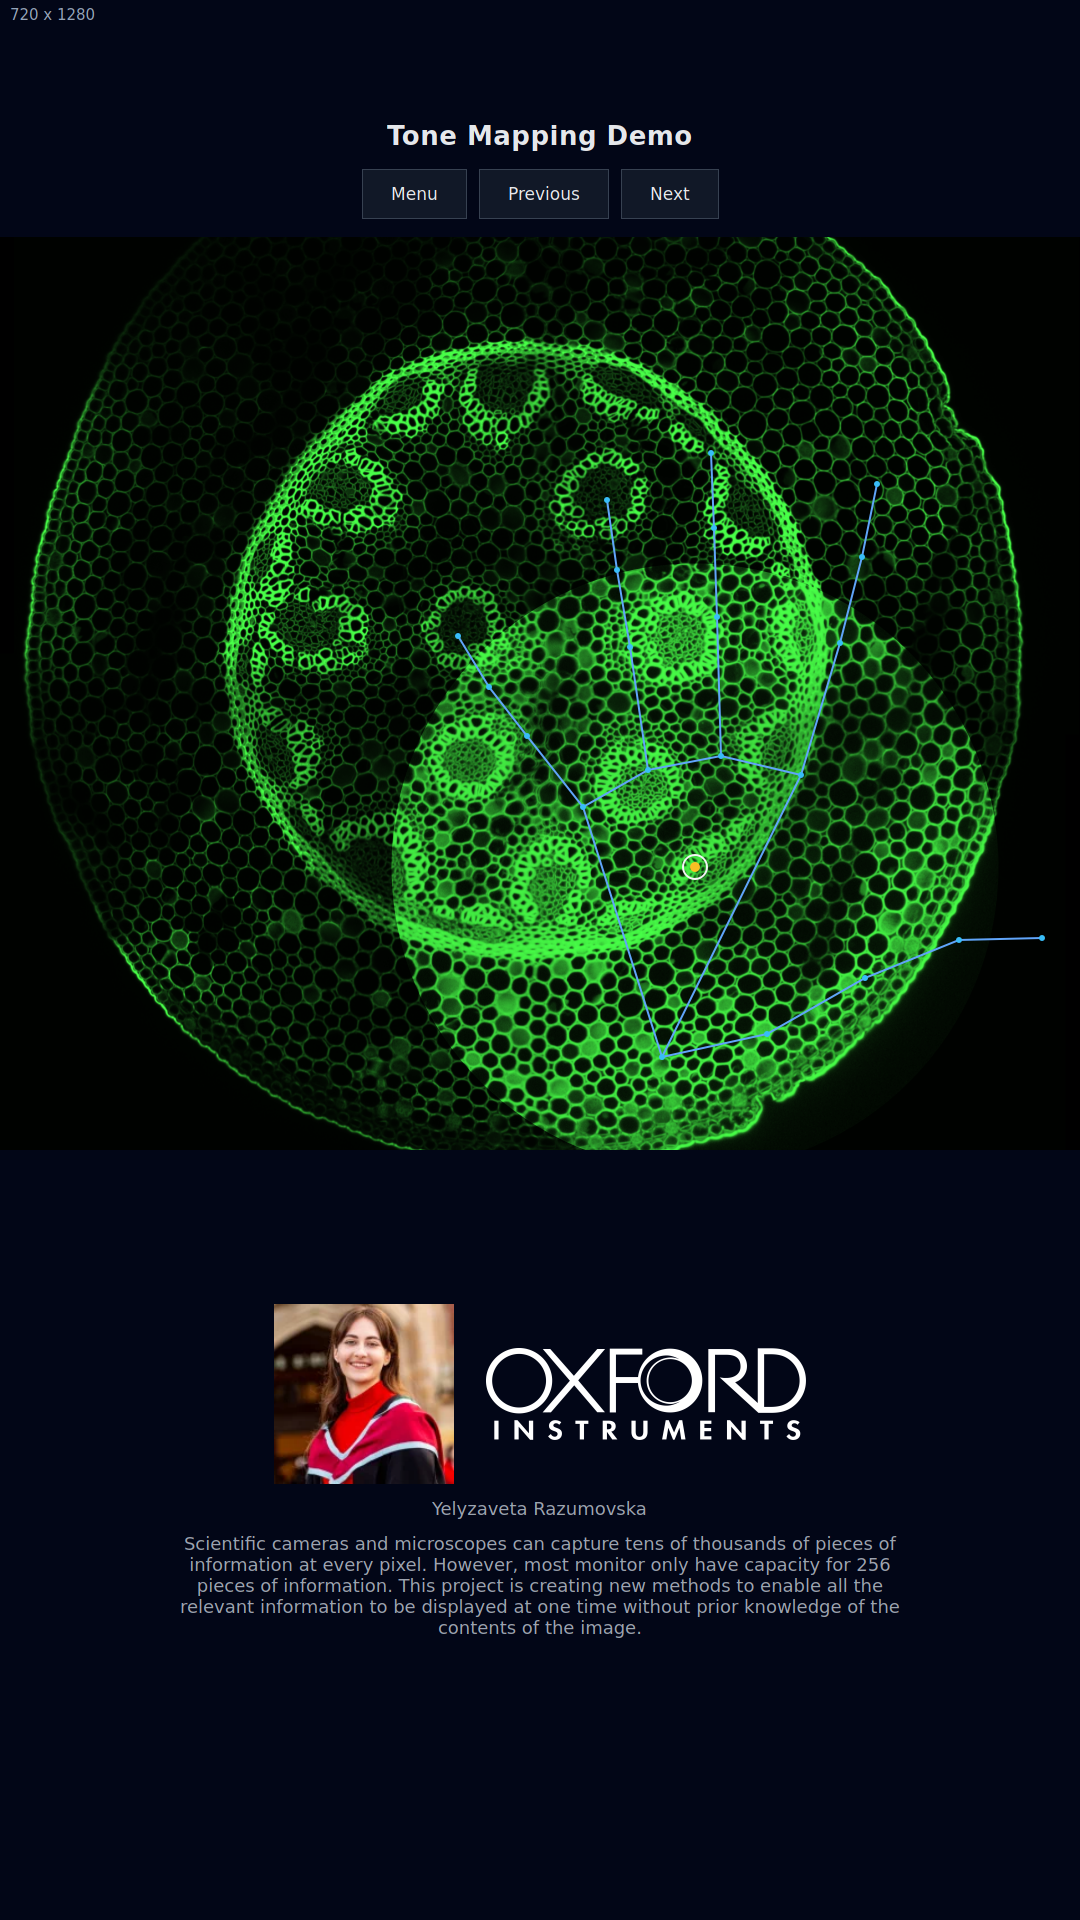
\includegraphics[width=0.31\textwidth]{Screenshot from 2026-04-23 21-33-14.png}
    \hfill
    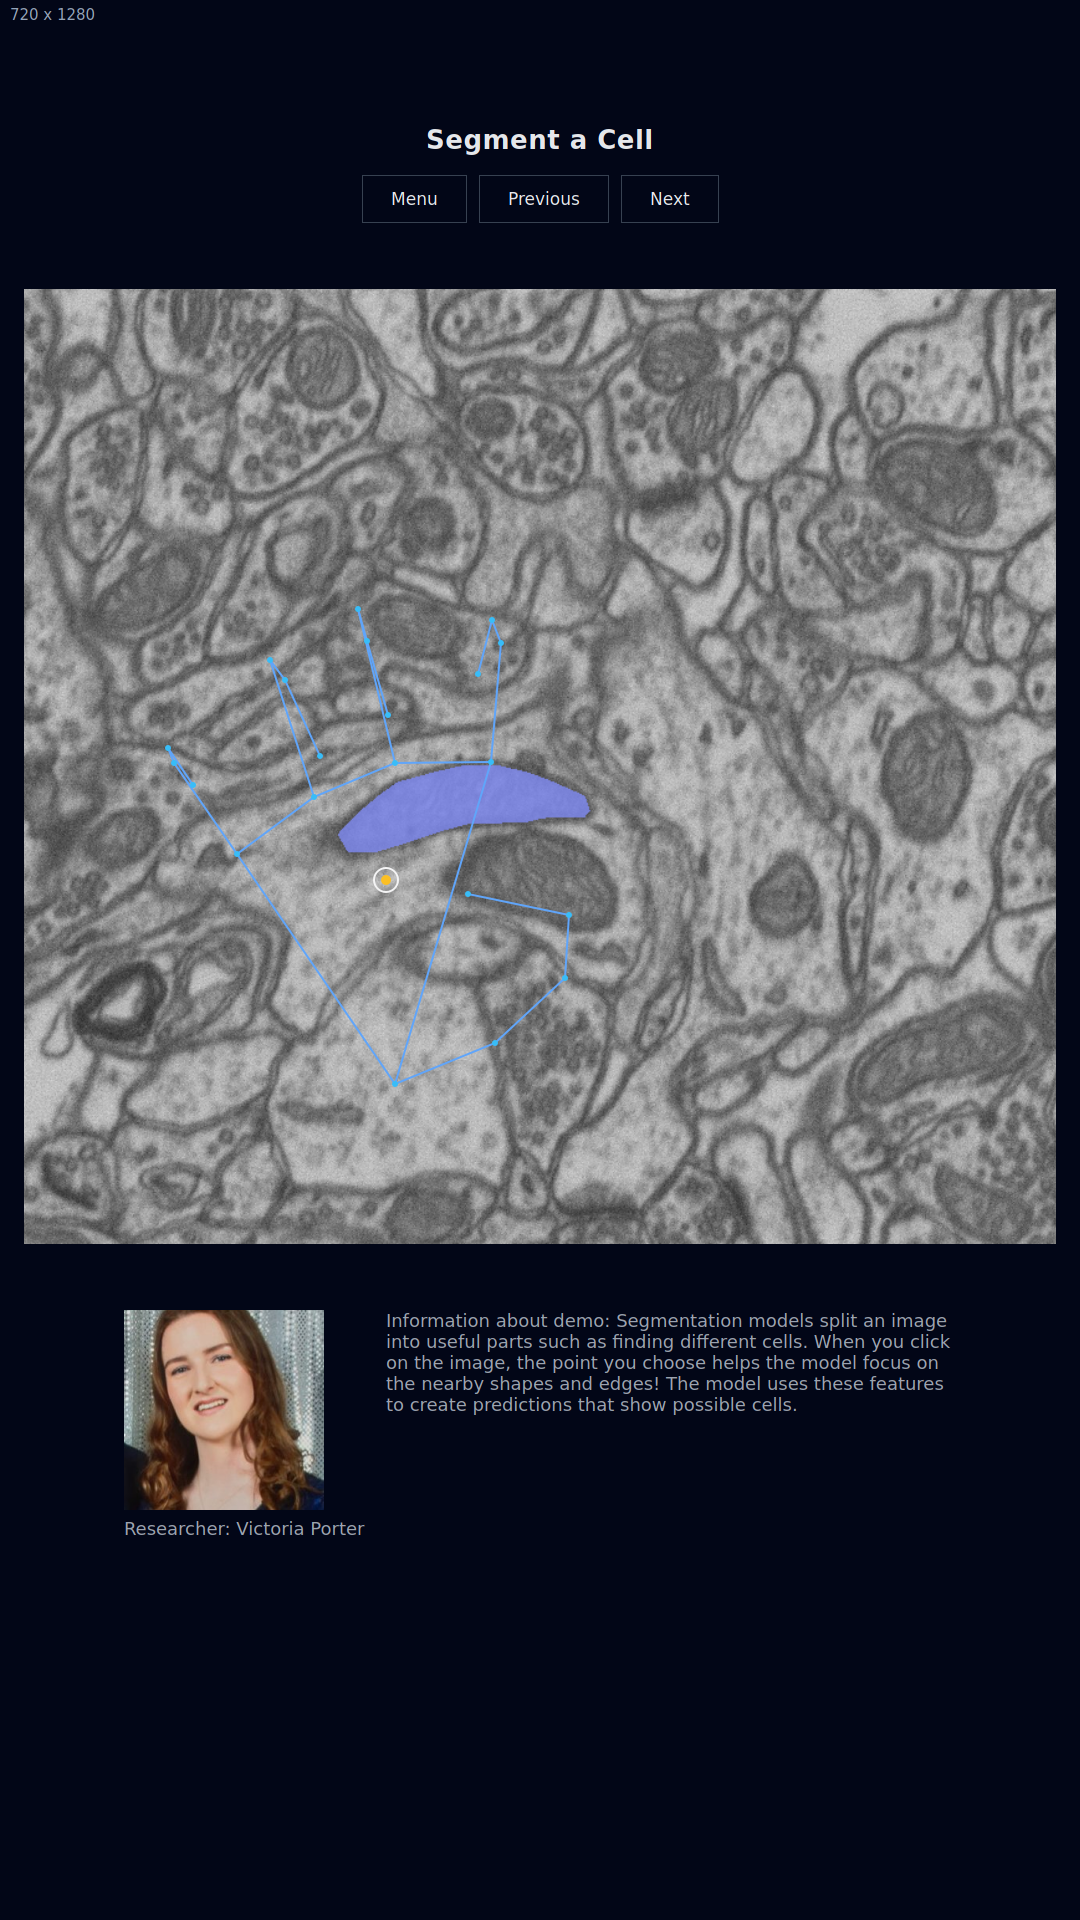
\includegraphics[width=0.31\textwidth]{Screenshot from 2026-04-23 21-33-54.png}
    \caption{These screenshots show representative screens from the implemented gesture-controlled user interface.}
    \label{fig:ui-screens}
\end{figure}

\subsubsection{Quality Assurance Steps}

\paragraph*{Version Control and Versioning}

Development of the demonstrator was managed through Git-based version control.
This made it possible to track changes to the application logic,
documentation, and bundled assets while the interaction model and
presentation flow were still being refined.

\paragraph*{Code Style and Convention}

Although the demonstrator is implemented largely in a single file, a
consistent internal structure was used to keep the code understandable.
Configuration constants are grouped near the top of the file, helper
functions implement the gesture calculations, dedicated widget classes
encapsulate the different demo views, and the \texttt{MainWindow} class
coordinates page flow and interaction state. Descriptive naming and
lightweight inline documentation were used to keep the behaviour clear during
development.

\appendix

\section{Appendices}

\subsection{Supervisor Meeting Minutes}

The following minutes are presented in concise form and record a brief summary
of each meeting, the matters discussed, and the agreed actions.

\subsubsection*{2025-10-08}

Summary: Initial project-scoping meeting.
Discussed: lightweight hand pose tracking for real-time HCI on edge hardware,
possible use of RGB and stereo input, and the need for an early literature
review.
Actions agreed: begin literature review, identify core papers, and prepare an
initial problem statement.

\subsubsection*{2025-10-14}

Summary: Follow-up meeting on early literature findings.
Discussed: latency versus accuracy on edge devices, candidate hardware, and how
pose quality would relate to HCI usability.
Actions agreed: continue literature review, shortlist likely baselines and
datasets, and start outlining the preliminary article.

\subsubsection*{2025-10-21}

Summary: Reported progress on an exploratory hand-tracking mini project.
Discussed: using a ZED camera and MediaPipe Hands to gain practical experience
with hand-tracking behaviour, including lighting, range, and gesture stability.
Actions agreed: continue the exploratory demo as hands-on domain familiarisation
while keeping it separate from the main research contribution.

\subsubsection*{2025-10-28}

Summary: Reviewed exploratory demo progress and article direction.
Discussed: practical constraints observed in camera-based hand interaction and
how these could inform the motivation for the project.
Actions agreed: draft the introduction and motivation sections and continue the
structured literature review.

\subsubsection*{2025-11-04}

Summary: Literature review review meeting.
Discussed: MediaPipe Hands, lightweight hand-pose approaches, stereo or
depth-related methods, and how to position the project around edge HCI rather
than model accuracy alone.
Actions agreed: deepen the review, organise references, and continue drafting
the preliminary article.

\subsubsection*{2025-11-11}

Summary: Discussed the developing preliminary article.
Discussed: project framing around lightweight hand pose tracking for edge
devices, likely hardware and sensing setup, and the need to state clear
objectives.
Actions agreed: refine the abstract and research aim and improve the structure
of the literature review.

\subsubsection*{2025-11-18}

Summary: Progress review before the preliminary submission.
Discussed: draft introduction and literature review, possible evaluation themes
such as latency, stability, and usability, and how much preliminary
implementation to mention.
Actions agreed: complete a near-final draft of the preliminary article and
prepare the progress appendix.

\subsubsection*{2025-12-02}

Summary: Final pre-submission review before the preliminary article deadline.
Discussed: article structure, wording of the objectives, literature coverage,
and the role of the exploratory demo as early practical work.
Actions agreed: make final edits, proofread, and submit the preliminary
research article by 2025-12-05.

\subsubsection*{2025-12-15}

Summary: Post-submission review after the preliminary article.
Discussed: lessons from the initial phase, narrowing the project to a more
deliverable software artefact, and possible next implementation steps.
Actions agreed: define a clearer implementation plan and prepare for the main
development phase over the break.

\subsubsection*{2026-01-06}

Summary: Restart meeting after the winter break.
Discussed: refining scope from a broad stereo/RGB investigation toward a more
manageable core system with reproducible software and evaluation.
Actions agreed: define the main implementation scope, organise the repository,
and begin the next development phase.

\subsubsection*{2026-01-13}

Summary: Reviewed software architecture direction.
Discussed: reusable package structure, scripts for training, evaluation and
inference, likely datasets, and the importance of a strong baseline.
Actions agreed: implement the core project structure and begin assembling the
training and evaluation workflow.

\subsubsection*{2026-01-20}

Summary: Reported progress on codebase setup.
Discussed: package organisation, dataset handling, checkpointing, and the need
to keep the system reproducible and well documented from an early stage.
Actions agreed: continue the core implementation and validate the basic
training and inference path.

\subsubsection*{2026-02-03}

Summary: Model-development review meeting.
Discussed: adopting a DRHand-inspired direction, staged training, loss design,
and balancing technical ambition with a feasible implementation.
Actions agreed: proceed with the selected architecture, document assumptions,
and begin controlled experiments.

\subsubsection*{2026-02-17}

Summary: Reviewed early implementation and evaluation progress.
Discussed: training behaviour, checkpoint management, evaluation scripts, and
the importance of preserving reproducible outputs for the final reports.
Actions agreed: continue experiments, improve workflow robustness, and preserve
representative outputs.

\subsubsection*{2026-02-24}

Summary: Intermediate results review.
Discussed: practical performance of the current pipeline, comparison against
baseline ideas, and how to connect the software work back to the edge-HCI
motivation.
Actions agreed: continue evaluation, improve result organisation, and begin
outlining the final research and software reports.

\subsubsection*{2026-03-03}

Summary: Focus on implementation maturity and supporting infrastructure.
Discussed: evaluation outputs, benchmarking, reproducibility, and the role of
supporting software beyond the core model.
Actions agreed: improve scripts, artefact management, and documentation, and
prepare report-ready material.

\subsubsection*{2026-03-10}

Summary: Shifted attention toward the Software Development Report.
Discussed: report structure, architecture description, quality-assurance
material, and what evidence should be included for testing and documentation.
Actions agreed: draft software report sections and ensure the repository
documentation supports installation and reuse.

\subsubsection*{2026-03-16}

Summary: Reviewed final-report and presentation preparation.
Discussed: research article drafting, software report content, presentation
planning, and how the earlier interactive demo could be described as a
companion exploratory artefact.
Actions agreed: continue writing, refine the software documentation, and
prepare material suitable for the final demonstration and slides.

\subsubsection*{2026-03-25}

Summary: Final major supervision meeting before the submission run-in.
Discussed: remaining writing tasks, repository documentation, appendix
material, and preparation for the 2026-04-27 deadlines for the research
article, software development report, and presentation slides.
Actions agreed: complete final experiments and writing, finalise the repository
documentation set, prepare the presentation, and assemble the appendices for
submission.

\end{document}
